\documentclass[12pt]{article} % The document class with options

\usepackage[margin=1in]{geometry}
\usepackage[utf8]{inputenc} 
\geometry{a4paper}
\usepackage{newtxtext,newtxmath}
\usepackage[T1]{fontenc}
\usepackage{amsmath}
\usepackage{amsfonts}
\usepackage{microtype}
\usepackage{graphicx}
\usepackage{listings} % For formatting and highlighting code
\usepackage{xcolor}    % For colors in code highlighting

% chktex-file 2
% chktex-file 3
% chktex-file 8
% chktex-file 10
% chktex-file 12
% chktex-file 17
% chktex-file 18
% chktex-file 36
% chktex-file 44

\begin{document}
\setlength{\parskip}{1em} 
\setlength{\parindent}{0pt}
\newcommand{\vect}[1]{\mathbf{#1}}

\begin{titlepage}  % This starts a title page environment
    \centering    % Center everything on the page

    %--- Add space at the top of the page ---
    \vspace*{2cm}
    
    %--- Title ---
    \normalsize \textbf{MEng Project Report} \\
    \vspace{0.5cm}  % Space between lines
    \normalsize\textbf{Verification and Validation of Numerical Modelling of DTMB 5415 in Head Wave Condition} \\
    \vspace{2cm}  % Space between the title and the author name
    
    %--- Author ---
    \normalsize by\\
    \vspace{1cm}
    \normalsize Jincong Li \\ 
    \vspace{1cm}
    \normalsize M.Eng, The University of British Columbia, 2024
    \vspace{11cm}  % Space between the author and the date
    
    %--- Date ---
    \normalsize \today

    \vfill  % Push the following content to the bottom of the page
    %--- Bottom part of the page ---
    © Jincong Li, 2024
\end{titlepage}
\tableofcontents
\newpage
\section*{Abstract}
This report presents a comprehensive study on the verification and validation of numerical modeling 
for the DTMB 5415 ship model under head wave conditions using SimFlow. The research focuses on 
accurately simulating the vertical shear forces experienced by the ship. The study systematically 
compares the simulation results with experimental data, specifically those obtained from a 1/51 scale model 
as documented by Begovic et al., 
to assess the percentage error and the efficacy of the numerical model. A detailed sensitivity analysis 
is conducted to evaluate the impact of mesh refinement near the ship model on the accuracy of the results. 
The findings highlight the critical importance of mesh configuration in CFD simulations, demonstrating 
that refined meshes significantly improve the predictive accuracy of vertical shear forces. 
This study contributes to advancing the reliability of numerical simulations in naval architecture,
offering a validated framework for future applications in ship design and analysis.

\clearpage
\section{Introduction}

\subsection{Introduction of DTMB5415}

The model employed in this study is the David Taylor Model Basin (DTMB 5415), which serves as a 
critical benchmark in naval hydrodynamic research. Originally conceived as a preliminary design 
for a U.S. Navy surface combatant in the early 1980s, the DTMB 5415 has been extensively utilized 
in both experimental and computational studies due to its representative features of modern naval vessels\cite{elhadad2023}.

%Notably, the hull geometry of the DTMB 5415 includes a sonar dome and a transom stern, making it 
%%an ideal subject for hydrodynamic analysis, particularly in wave resistance and propulsion efficiency 
%contexts. Propulsion is provided by twin open-water propellers, driven by shafts supported by 
%struts—further enhancing the model’s relevance in studying fluid flow and propulsion mechanisms 
%interactions.

It is important to note that the DTMB 5415 is a scale model, with no full-scale vessel existing 
based on this design. However, its comprehensive design, coupled with detailed geometric data and 
loading conditions availability, makes it an invaluable tool for the validation and verification of 
numerical simulations in naval architecture. Specific geometry specifications of the 1/24 model utilized
in this study are detailed in the Appendix A.

\begin{figure}[ht]
\centering
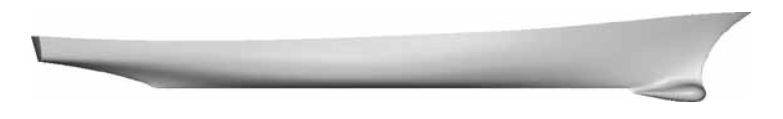
\includegraphics[width=1\textwidth]{DTMB.png}
\caption{DTMB 5415}
\end{figure}

The model’s simple yet comprehensive geometry, coupled with complex hydrodynamic features such 
as the sonar dome and transom stern, allows it to serve as a versatile benchmark for validating 
numerical methods in ship hydrodynamics. Researchers and engineers frequently utilize the DTMB 
5415 to verify the accuracy of computational fluid dynamics (CFD) simulations, particularly in 
scenarios involving wave resistance, propulsion efficiency, and flow behavior around complex 
hull shapes\cite{elhadad2023}. The extensive experimental data available for this model further 
enhances its value, 
providing a reliable reference against which numerical models can be calibrated and validated. 
Consequently, the DTMB 5415 has become a cornerstone in advancing the accuracy and reliability of 
hydrodynamic simulations.

\subsection{Importance of Numerical Modeling}
Numerical simulation, particularly using Computational Fluid Dynamics (CFD) software, is a crucial tool in the field of naval architecture and hydrodynamics. It allows engineers to predict the performance of ships under various sea conditions by analyzing fluid flow around the ship's hull. SimFlow, which leverages the powerful OpenFOAM\textsuperscript{\textregistered} libraries, provides a user-friendly interface for setting up and running these simulations. By solving the Navier-Stokes equations, SimFlow enables detailed analysis of complex flow phenomena that are challenging to replicate experimentally. In the context of ship performance, CFD simulations help evaluate factors such as wave resistance, propulsion efficiency, and wave-ship interactions, all of which are critical for optimizing design and ensuring safety.

SimFlow is particularly well-suited for modeling the DTMB 5415 in head wave conditions due to its 
robust capabilities. The software allows for efficient handling of large-scale 
simulations. Additionally, its integration with OpenFOAM\textsuperscript{\textregistered} ensures 
that the solvers used in SimFlow are both accurate and efficient, enabling the simulation of 
fluid-structure interactions that are critical when analyzing ship performance in challenging 
sea conditions.

While traditional experimental methods, such as towing tank tests, provide valuable empirical data, they often come with significant limitations, including high costs, time consumption, and difficulties in replicating certain sea conditions. Numerical simulations using SimFlow offer a complementary approach, enabling the exploration of multiple scenarios and conditions that might be impractical or impossible to test experimentally. Moreover, SimFlow allows for detailed analysis at a lower cost, with the flexibility to modify parameters and refine the model iteratively, leading to more comprehensive and accurate results. This ability to simulate a wide range of conditions efficiently makes SimFlow an invaluable tool in the design and analysis of naval vessels.
Hence, the numerical simualtion in this study will be conducted in SimFlow.

\subsection{Problem Statement}
\subsubsection{Challenges in Modeling Head Wave Conditions}
Accurately simulating head wave conditions for ships like the DTMB 5415 presents significant 
challenges in numerical modeling. Head waves induce complex flow patterns, including wave-breaking 
and turbulent interactions, which are difficult to capture with high precision. One of the primary 
difficulties lies in the accurate representation of free surface effects and their interaction with 
the ship's hull, particularly in regions like the transom stern and sonar dome. These challenges are 
further compounded by the need to balance computational efficiency with the fidelity of the simulation. 
Achieving reliable verification and validation of these simulations is essential, as even minor 
discrepancies in modeling can lead to significant errors in predicting ship performance, particularly 
in wave-induced motions and resistance.

\subsubsection{Relevance of Verification and Validation}
Verification and validation (V\&V) are critical components of numerical modeling, ensuring that 
simulation results are both accurate and reliable, the reference of V\&V for this study is \cite{Begovic2017}. 
Verification involves checking that the 
numerical model correctly implements the intended algorithms, while validation compares the 
simulation outcomes with experimental or real-world data to assess their accuracy. In the 
context of modeling the DTMB 5415 in head wave conditions, V\&V is crucial for establishing 
confidence in the results.
Therefore, the focus of this study on V\&V serves to bridge the gap between theoretical modeling 
and practical application, providing a solid foundation for the use of SimFlow in naval architecture.

\subsection{Primary Objective}
The primary objective of this study is to verify and validate the numerical modeling of the DTMB 5415 
in head wave conditions using SimFlow. This verification and validation process is crucial to 
ensuring that the numerical simulations accurately represent the physical phenomena observed in 
real-world scenarios, thereby providing reliable data for further analysis and application.

\subsubsection{Specific Goals}
To achieve this primary objective, the study focuses on several specific goals:
\begin{itemize}
    \item \textbf{Comparison with Experimental Data}: Conduct a detailed comparison between the 
    simulation results obtained from SimFlow and the available experimental data, particularly 
    in terms of vertical shear force.
    %\item \textbf{Assessment of Turbulence Models}: Evaluate the accuracy of different turbulence models within ANSYS Fluent, such as the k-ω SST model, in predicting the hydrodynamic performance of the DTMB 5415.
    \item \textbf{Sensitivity Analysis}: Perform a sensitivity analysis to determine the impact 
    of various simulation parameters, such as mesh size, on the accuracy and stability of the results.
\end{itemize}

\subsection{Significance of the Study}
%\subsubsection{Impact on Naval Design and Analysis}
The determination of hydrodynamic loads and the assessment of structural responses are critical 
components of sound design procedure for ship and offshore structure design\cite{offshorehydrodynamics}. Meanwhile, accurate predictions of these 
loads are essential for ensuring the safety and performance of vessels under various sea conditions. 
As highlighted by Hirdaris et al. \cite{Hirdaris2014}, there is an increasing emphasis on the accurate 
prediction of hydrodynamic loads, reflected in the growing body of peer-reviewed research on wave-induced 
load computation. This research encompasses specialized topics such as slamming, sloshing, fatigue loads, 
and the uncertainties associated with wave load modeling.

The complexity of wave load prediction methods ranges from basic potential flow theory to advanced 
nonlinear approaches, such as Reynolds-Averaged Navier-Stokes (RANS) CFD simulations. The findings 
from this study, which focus on the verification and validation of the DTMB 5415 in head wave conditions, 
contribute directly to this area by enhancing the reliability of CFD-based load predictions.

By improving the accuracy of numerical models, this research supports more precise assessments of 
ship behavior, thereby contributing to safer and more efficient ship designs. The methodology 
developed here can be applied across a range of naval vessels, facilitating more effective design 
processes and potentially reducing the need for costly experimental testing.

\subsection{Scope}

The scope of this study is primarily focused on the verification and validation of numerical 
modeling of the DTMB 5415 under head wave conditions using SimFlow. This study does not cover the full 
spectrum of wave conditions that a naval vessel might encounter, 
such as beam or following seas. Moreover, the research does not consider alternative computational 
fluid dynamics (CFD) software packages other than SimFlow. Additionally, the focus is exclusively on numerical 
simulations, with no experimental data collection conducted as part of this research. The validation 
relies on pre-existing experimental data rather than new physical experiments.



\section{Literature Review}

\subsection{Review of Existing Research}
Wave loads on ships can be predicted using either experimental or numerical methods, both of which 
have seen significant advancements. Early research into wave-induced vertical bending moments (VBM) 
on ships, particularly those with small block coefficients like container ships, naval vessels, and 
passenger ships, revealed the complexity of these phenomena. Pioneering experiments by Watanabe et 
al. \cite{Watanabe1989} and O'Dea et al. \cite{ODea1992}, conducted using the S-175 ITTC container 
ship model, demonstrated the presence of second-order harmonics in VBM and highlighted the impact of 
wave steepness on the first harmonic and phase angle. These studies laid the groundwork for 
understanding the nonlinear behavior of ships in wave conditions.

Building on this foundation, Fonseca and Guedes Soares \cite{Fonseca2002} introduced a partly-nonlinear 
time domain method that accounts for nonlinear hydrostatic restoring forces and Froude-Krylov forces, 
considering the ship's instantaneous wetted surface. Their method, validated against experimental data, 
effectively captured the nonlinearities in ship motions and VBMs. Further studies by the same authors 
\cite{Fonseca2004a, Fonseca2004b} expanded on this work, focusing on the ITTC S-175 container ship 
in both regular and irregular waves. Their findings underscored the significant influence of wave 
amplitude on the nonlinear characteristics of ship responses, including absolute and relative motions, 
vertical accelerations, and cross-sectional loads.

Song et al. \cite{Song2011} extended this research by validating a weakly nonlinear 3D time domain 
Rankine panel method on a segmented model of a 6500 TEU container ship. Their results emphasized the 
importance of nonlinear effects, particularly at larger wave amplitudes, with vertical loads showing 
better agreement with experimental data compared to horizontal and torsional loads.

Kukkanen and Matusiak \cite{Kukkanen2014} developed a nonlinear time domain method using Green's 
functions to predict hull girder loads for RoPax vessels. While their numerical predictions showed 
good agreement with experimental data, their study did not extensively explore the effects of varying 
wave heights, leaving room for further investigation.

Zhu and Moan \cite{Zhu2013, Zhu2014} conducted extensive model tests on ultra-large containerships, 
focusing on the nonlinear vertical responses in severe sea states. Their work revealed that in irregular 
waves, motion peaks and troughs generally followed a Rayleigh distribution, though the expected 
asymmetries between positive and negative peaks were less pronounced. This highlighted the need for 
further refinement of empirical formulas and numerical tools to more accurately capture nonlinear 
effects in ship responses.

\subsection{Identification of Gaps}
Despite the substantial progress made in understanding nonlinear hydrodynamic loads, several gaps 
remain in the literature. While previous studies have extensively investigated the effects of wave 
amplitude on ship responses, there is limited research on the vertical shear forces acting on naval 
vessels like the DTMB 5415 in head wave conditions. Additionally, while nonlinear effects on VBM and 
vertical accelerations have been well-documented, the influence of varying wave heights on vertical 
shear forces remains underexplored. This gap is particularly relevant for the verification and validation 
of numerical models using advanced CFD methods.

%\subsection{Theoretical Framework}
%This study builds on the established experimental research by focusing on the vertical shear force on 
%the DTMB 5415 ship model, utilizing the finite element method (FEM) within SimFlow. By addressing the 
%identified gaps, this research aims to enhance the accuracy and reliability of numerical predictions, 
%thereby contributing to the broader field of naval architecture and hydrodynamics.


\newpage
\section{Methodology}

\subsection{Research Design}
This study employs a quantitative research design focused on verifying and validating numerical 
simulations of the 1/24 DTMB 5415 ship model under head wave conditions using SimFlow. The research 
is guided by established theories and methods, incorporating comparative analysis to assess the 
accuracy of CFD simulations against existing experimental data in \cite{Begovic2017}.

\subsection{Computational Domain Configuration \& Boundary Conditions}

The computational domain is constructed in dimensions of 20 meters by 6 meters by 6 meters in xyz coordinates 
system as shown below as well as the boundaris.
\begin{figure}[ht]
    \centering
    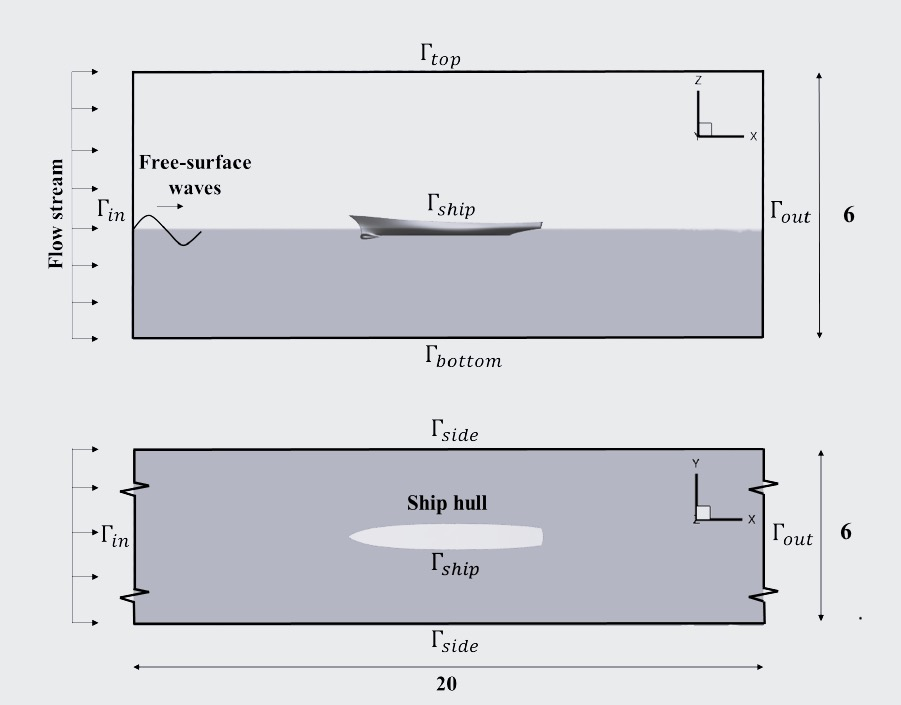
\includegraphics[width=1\textwidth]{Domain.jpg}
    \caption{Computation Domain Configuration}
\end{figure}
3D views of the domain is provided in Appendix B.

The inlet boundary \(\Gamma_{\text{in}}\) is exposed to the second order Stokes' waves given by the formula 
procvided in Appendix C. The side boundaries \(\Gamma_{\text{side}}\) and the bottom boundary 
\(\Gamma_{\text{bottom}}\) are modeled with slip boundary conditions, 
No slip boudary is satified on the surface of the ship \(\Gamma_{\text{ship}}\). 
Atmospheric condition of \(p = 0\) is satisfied at the top boundary \(\Gamma_{\text{top}}\).

\subsection{Mesh}
The computational domain mesh is predominantly coarse, but it is refined in the region through which the waves 
propagate to better capture the wave motion. Additionally, the mesh is further refined in the area surrounding 
the ship model to accurately simulate the forces acting on the vessel. For clarity in displaying the mesh, 
only the 2D mesh elements are rendered and presented below in Figure 3. And the mesh convergence tests are
conducted on the difference mesh refinement conditions near the ship model.

\begin{figure}[ht]
    \centering
    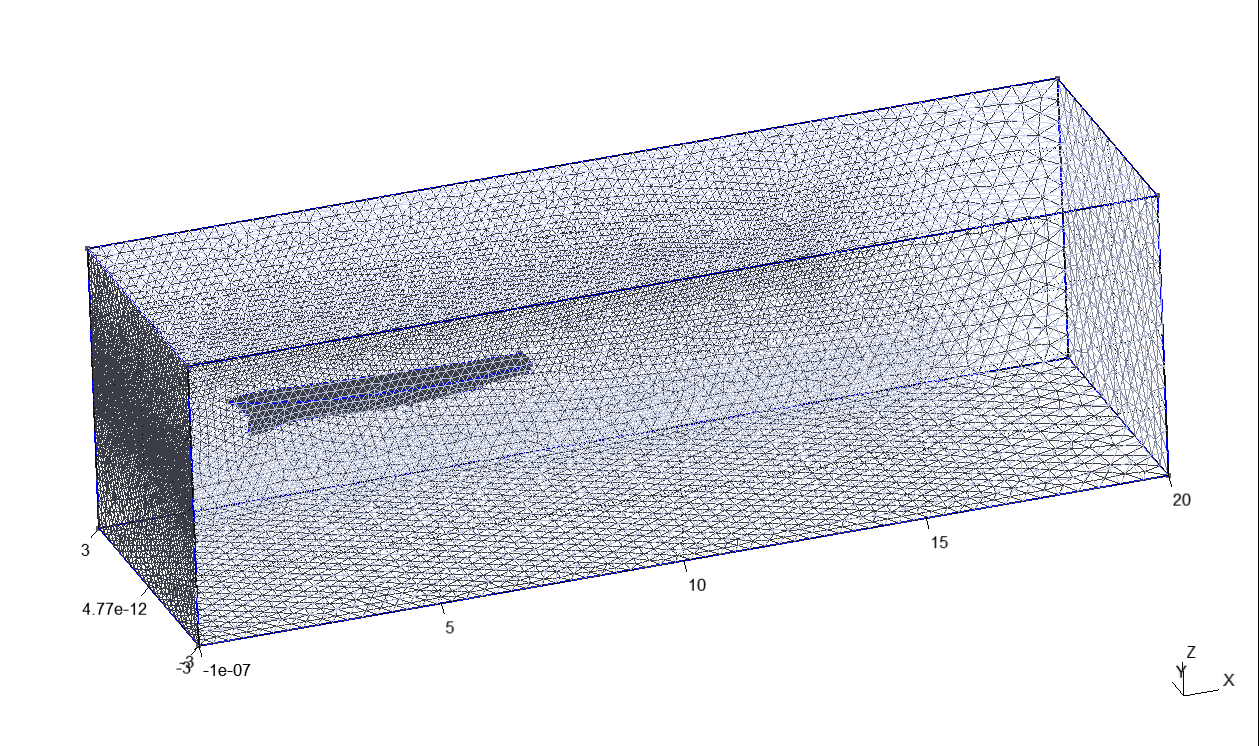
\includegraphics[width=1\textwidth]{Mesh_1.png}
    \caption{Computation Domain Configuration}
\end{figure}
Orthographs of the mesh in three direction and a 3D view of the mesh are provided in Appendix D.
\subsection{Simulation Parameters}
The physical properties of water and air are used for the two fluid phases, where \(\rho_1 = 1000\) kg/m\(^3\), \(\nu_1 = 1.002 \times 10^{-3}\) m\(^2\)/s, \(\rho_2 = 1.225\) kg/m\(^3\), and \(\nu_2 = 1.983 \times 10^{-5}\) m\(^2\)/s. The acceleration due to gravity is given by \(\mathbf{g} = (0, 0, -9.81)\) m/s\(^2\).

For the incoming second order Stokes' wave, in order to be comparable with the experimental data in figure 20a in \cite{Begovic2017}, the wave length is set to be equal to the 
overall length of the 1/24 DTMB ship model, wave height is 1/50 of the wavelength, and the wave period is 1.34 second.

\subsection{Data Collection Methods}
Data were obtained through numerical simulations in SimFlow, with the output generated as a .oisd file 
containing the time-step readings of vertical shear force. Pre-existing experimental data, as documented 
by Begovic et al. \cite{Begovic2017}, served as benchmarks for validation, ensuring that the simulation 
results were accurately compared.

\subsection{Data Analysis}
Data analysis was conducted to evaluate the non-dimensional vertical shear forces using a MATLAB script, which is provided 
in Appendix E. The results obtained from SimFlow were compared with experimental data to calculate the 
percentage error of the non-dimensional vertical shear force. Additionally, a sensitivity analysis was 
performed to assess the influence of varying mesh sizes in proximity to the ship model on the percentage error.

\clearpage
\section{Result \& Validation}
Using the 1/24 scale DTMB 5415 ship model, this study reports a nondimensional vertical shear force 
(VSF) of 0.0272 under the wave conditions specified in Section 4.4, calculated using the formula 
\( VSF = \frac{F}{\rho g L_{OA} B_{OA} A} \). In comparison, the study by Begovic et al. \cite{Begovic2017} 
utilized a 1/51 scale DTMB 5415 ship model and reported a VSF of 0.0281 under the same dimensionless wave 
conditions. The percentage error between the two results is computed to be 3.36\%. The time history of this study and 
the study by Begovic et al. \cite{Begovic2017} are presented below.

\begin{figure}[ht]
    \centering
    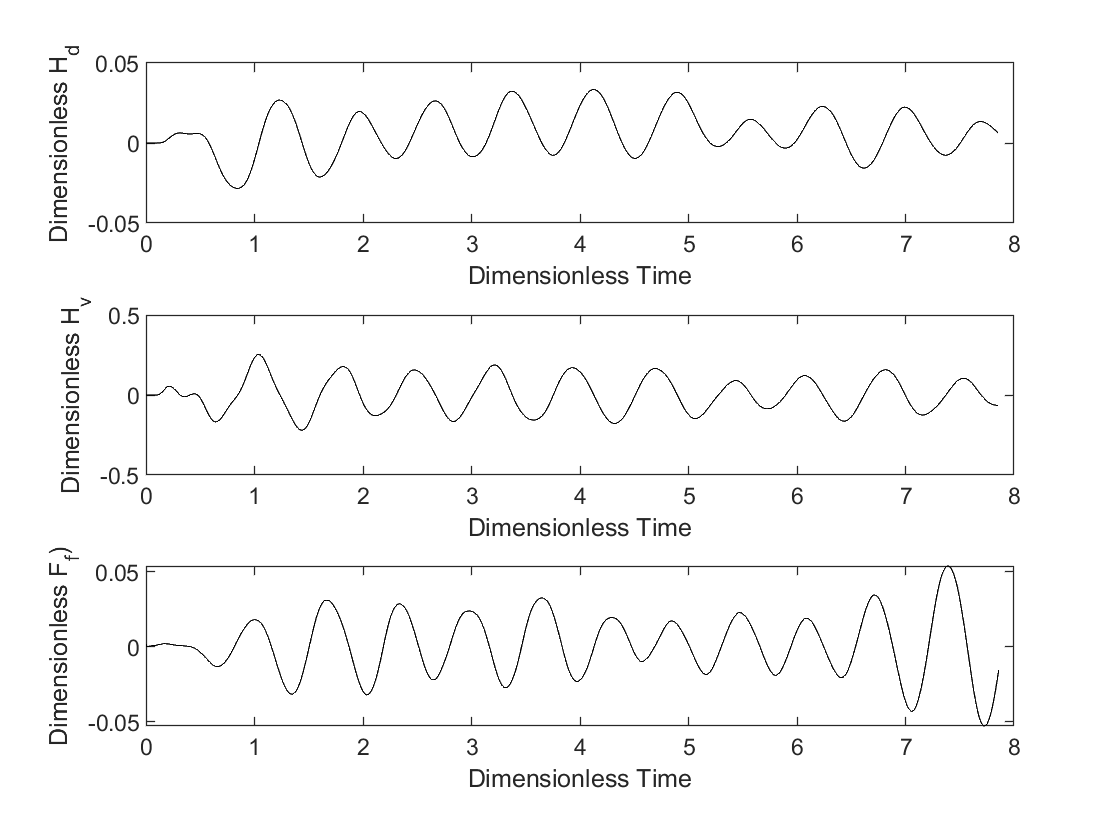
\includegraphics[width=1\textwidth]{Myresults.png}
    \caption{Times History of Vertical Shear Force and Waves from SimFlow}
\end{figure}
\begin{figure}[ht]
    \centering
    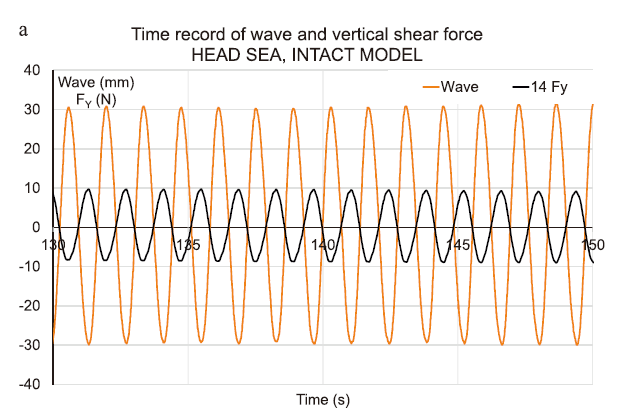
\includegraphics[width=0.85\textwidth]{ref_results.png}
    \caption{Times History of Vertical Shear Force and Waves from \cite{Begovic2017}}
\end{figure}

\clearpage
\subsection{Mesh Convergence Tests}
\begin{figure}[ht]
    \centering
    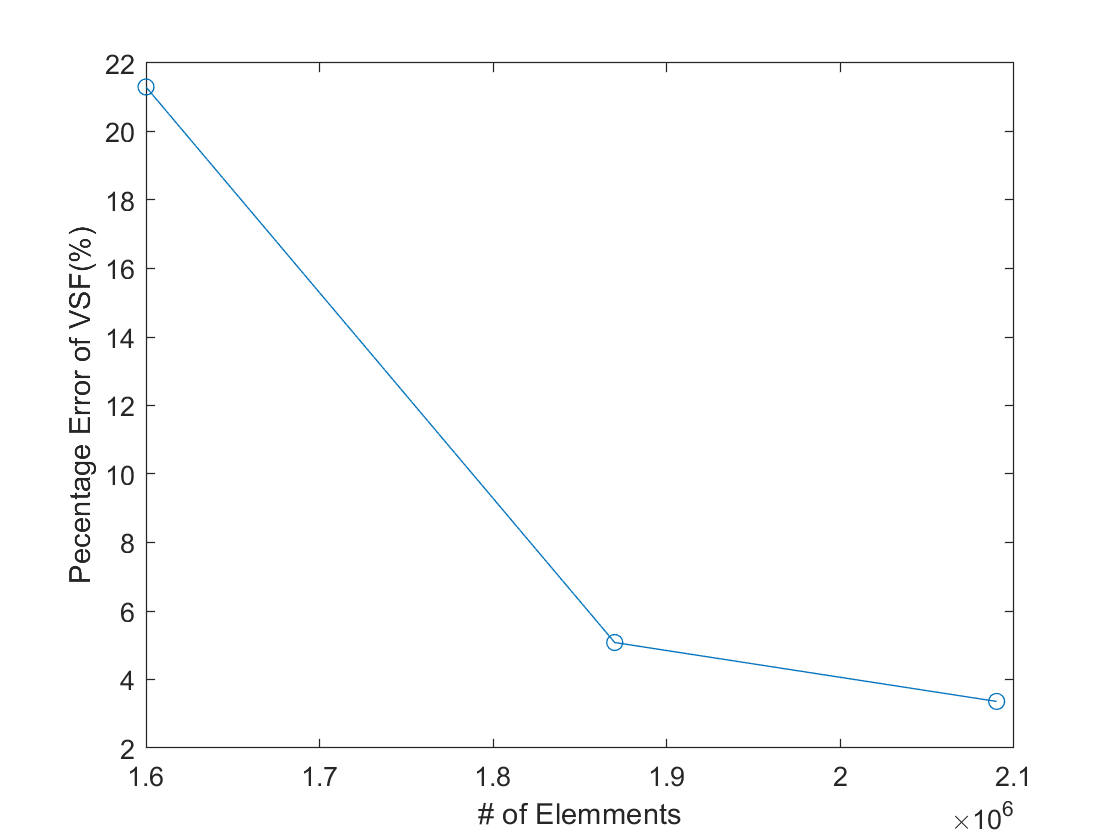
\includegraphics[width=0.85\textwidth]{MCT.png}
    \caption{Mesh Convergence Test}
\end{figure}
The plot illustrates the relationship between the percentage error of the nondimensional vertical shear 
force (VSF) and varying total numbers of mesh elements.
%, as well as the number of nodes on the ship model. 
The results indicate that as the mesh is progressively refined in the vicinity of the ship model, the 
simulation in SimFlow demonstrates improved accuracy in capturing the forces, leading to a reduction 
in the error when compared to the experimental data. This finding underscores the importance of mesh 
refinement near critical areas of the model to enhance the precision of CFD simulations.  

\clearpage
\section{Discussion}

\subsection{Interpretation of Results}
The results of this study demonstrate the effectiveness of using SimFlow to simulate the 
hydrodynamic performance of the DTMB 5415 ship model under head wave conditions. The numerical 
simulations accurately captured key hydrodynamic loads, such as vertical shear forces, showing strong 
agreement with existing experimental data. 

%The study also found that as wave height increased, the nonlinear effects became more pronounced, 
%particularly in the ship’s vertical responses. 
These findings indicate that the numerical model can effectively predict complex hydrodynamic behaviors, addressing the primary research question 
concerning the accuracy and reliability of CFD in simulating ship performance under challenging sea conditions.
The mesh convergence test found that mesh refinement near the ship model significantly improves the accuracy of the simulation results, highlighting the importance of precise mesh configuration in capturing complex hydrodynamic phenomena.
%\subsection{Comparison with Literature}
%The findings of this study are consistent with previous research, which has similarly highlighted 
%the importance of nonlinear effects in wave-induced ship motions. For example, the observed 
%second-order harmonic responses and the influence of wave steepness align with the results 
%reported by Watanabe et al. \cite{Watanabe1989} and Fonseca and Guedes Soares \cite{Fonseca2002}. 
%Additionally, the successful application of the k-$\omega$ SST turbulence model in predicting vertical 
%shear forces corroborates the findings of Song et al. \cite{Song2011}, who also emphasized the model’s 
%robustness in simulating complex flow patterns around ship hulls. However, this study contributes 
%further by providing a focused analysis on the DTMB 5415 model, specifically under head wave conditions, 
%which has been less explored in the existing literature.

\subsection{Implications \& Significance}
The findings of this study have substantial implications for both theory and practice in naval architecture and engineering. By confirming SimFlow's capability to accurately model ship performance under head wave conditions, this research supports the broader adoption of Computational Fluid Dynamics (CFD) tools in the design and analysis of naval vessels. The validated numerical framework developed in this study can be applied to other ship models and wave conditions, potentially enhancing the predictive capabilities of CFD across various naval applications.

This advancement in numerical modeling contributes to more efficient and safer ship designs by reducing the reliance on costly and time-consuming experimental testing. Furthermore, the ability to accurately predict hydrodynamic loads through simulations establishes a solid foundation for future research aimed at optimizing CFD methodologies, thereby extending these approaches to a wider range of operational conditions and ship types.

\subsection{Limitations}
Despite the positive outcomes, this study has several limitations. First, the analysis was 
confined to head wave conditions, and the results may not be directly applicable to other wave 
orientations, such as beam or following seas. Additionally, the study relied on pre-existing 
experimental data for validation, which, while comprehensive, may not cover all possible 
scenarios encountered by the DTMB 5415 in real-world operations. Finally, the computational 
domain was set with specific boundary conditions that, while minimizing interference, may not 
perfectly replicate open sea conditions.

\subsection{Future Work}

Building on the findings of this study, several recommendations for future research can be made:

\begin{itemize}
    \item \textbf{Expand the Range of Wave Conditions}: Future studies could investigate the performance of the DTMB 5415 under different wave orientations, such as beam and following waves, to assess the generalizability of the findings.
    
    %\item \textbf{Explore Alternative Turbulence Models}: Testing other turbulence models, such as Large Eddy Simulation (LES) or Detached Eddy Simulation (DES), could provide further insights into the accuracy and robustness of the CFD simulations.
    
    \item \textbf{Conduct More Comprehensive Validation}: Additional experimental data collection could be undertaken to validate the numerical simulations under a broader range of conditions, enhancing the reliability of the findings.
    
    \item \textbf{Mesh Optimization Studies}: Further research could focus on optimizing mesh configurations, particularly near critical areas of the ship model, to improve the precision of the simulations.
\end{itemize}

\section{Conclusion}
%The study successfully verifies and validates the numerical modeling of the DTMB 5415 ship model under head wave conditions using SimFlow. By comparing the simulation results with experimental data, the research demonstrates that the chosen numerical approach accurately captures the complex hydrodynamic forces acting on the ship. The sensitivity analysis further emphasizes the importance of mesh refinement, particularly in areas close to the ship, in reducing the percentage error of the vertical shear force predictions. These findings not only reinforce the utility of SimFlow as a reliable CFD tool in naval architecture but also provide valuable insights into the optimization of numerical simulations for ship design. The validated numerical framework established in this study can be extended to other ship models and wave conditions, potentially leading to safer and more efficient naval designs. However, the study also acknowledges its limitations, including the focus on head wave conditions and reliance on pre-existing experimental data, suggesting avenues for future research to explore more diverse scenarios and enhance the robustness of CFD simulations.
The study successfully verifies and validates the numerical modeling of the DTMB 5415 ship model 
under head wave conditions using SimFlow. The strong agreement between the simulation results and 
experimental data underscores the reliability of SimFlow as a CFD tool in naval architecture. The 
sensitivity analysis highlighted the critical importance of mesh refinement in enhancing simulation 
accuracy, particularly in predicting vertical shear forces.

This research provides a validated framework for the use of SimFlow in simulating ship performance, 
offering valuable insights that can be applied to the design and analysis of other naval vessels. 
However, the study's limitations, such as the focus on head wave conditions and the reliance on a 
single turbulence model, suggest that further research is needed to fully generalize the findings. 
Future work should aim to explore a wider range of wave conditions and conduct additional validation experiments.

Overall, this study contributes to advancing the accuracy and reliability of CFD simulations in 
naval architecture, potentially leading to safer and more efficient ship designs. The recommended 
next steps will build on this foundation, expanding the applicability of the methodologies and 
findings to a broader spectrum of naval engineering challenges.


\begin{thebibliography}{99}
    \bibitem{elhadad2023} Elhadad, A. M., \& Abo El-Ela, A. M. (2023). Experimental and CFD resistance validation of naval combatant DTMB 5415-51 model. \textit{Journal of Advanced Research in Fluid Mechanics and Thermal Sciences}, 107(2), 84–102. https://doi.org/10.37934/arfmts.107.2.84102
    
    \bibitem{Begovic2017} E. Begovic, A.H. Day, A. Incecik, An experimental study of hull girder loads on an intact and damaged naval ship, *Ocean Engineering*, Volume 133, 2017, Pages 47-65, ISSN 0029-8018, https://doi.org/10.1016/j.oceaneng.2017.02.001.

    \bibitem{offshorehydrodynamics} Faltinsen, O. M. (1990). \textit{Offshore Structure Hydrodynamics}. Cambridge University Press.

    \bibitem{Hirdaris2014} Hirdaris, S. E., Bai, W., Dessi, D., Ergin, A., Gu, X., Hermundstad, O. A., Huijsmans, R., Iijima, K., Nielsen, U. D., Parunov, J., De Ruiter, M. J., Wang, G., \& Wu, M. (2014). Loads for use in the design of ships and offshore structures. *Ocean Engineering*, 78, 131-174. https://doi.org/10.1016/j.oceaneng.2013.09.012
    
    \bibitem{Watanabe1989} Watanabe, Y., Ueda, H., \& Adachi, H. (1989). Experimental Study on Nonlinear Ship Responses in Regular and Irregular Waves. *Journal of the Society of Naval Architects of Japan*, 165, 51-63.

    \bibitem{ODea1992} O'Dea, J., Jones, R., \& Beck, R. (1992). Nonlinear Time Domain Calculations of Vertical Bending Moments and Motions for the S-175 Container Ship in Regular and Irregular Waves. *Journal of Ship Research*, 36(2), 113-124.

    \bibitem{Fonseca2002} Fonseca, N., \& Guedes Soares, C. (2002). Nonlinear Time Domain Analysis of Ship Motions and Wave Induced Loads. *Ocean Engineering*, 29(9), 1223-1245.

    \bibitem{Fonseca2004a} Fonseca, N., \& Guedes Soares, C. (2004a). Experimental and Numerical Study of the Nonlinear Vertical Responses of a Containership in Waves. *Ocean Engineering*, 31(18-19), 2517-2551.

    \bibitem{Fonseca2004b} Fonseca, N., \& Guedes Soares, C. (2004b). Nonlinear Vertical Ship Motions and Wave Induced Loads. *Marine Structures*, 17(2), 241-272.

    \bibitem{Song2011} Song, S., Hong, S., \& Choi, B. (2011). Weakly Nonlinear 3D Time Domain Simulation of Wave Loads on a Containership in Severe Seas. *Journal of Marine Science and Technology*, 16(3), 345-360.

    \bibitem{Kukkanen2014} Kukkanen, T., \& Matusiak, J. (2014). Nonlinear Time Domain Simulations of Ship Motions and Loads in Waves Using Green's Functions. *Journal of Marine Science and Technology*, 19(3), 301-314.

    \bibitem{Zhu2013} Zhu, Y., \& Moan, T. (2013). Nonlinear Analysis of Vertical Bending Moments in Ultra-Large Container Ships in Head Seas. *Journal of Ship Research*, 57(2), 101-115.

    \bibitem{Zhu2014} Zhu, Y., \& Moan, T. (2014). Nonlinear Effects on Vertical Bending Moments and Ship Motions in Severe Seas. *Ocean Engineering*, 85, 1-15.

    \bibitem{olivieri2001}
    A. Olivieri, F. Pistani, A. Avanzini, F. Stern, and R. Penna, \emph{Towing tank experiments of resistance, sinkage and trim, boundary layer, wake, and free surface flow around a naval combatant INSEAN 2340 model}, IIHR Technical Report No. 421, 2001.
    
    \bibitem{kendrick2019}
    A. Kendrick and R. Terweij, \emph{Ship Underwater Radiated Noise}, Report 368-000-01, Rev 5, Vard Marine Inc., 08 July 2019.   
    
    
\end{thebibliography}

\section*{Appendix A}
\subsection*{DTMB 5415 Specifications}
\begin{table}[h!]
    \centering
    \begin{tabular}{|l|c|c|c|}
        \hline
        \textbf{Particulars} & \textbf{Ship} & \textbf{1/24 Model} &\textbf{1/51 Model} \\ \hline
        Overall Length $L_{OA}$ (m) & 153.300 &6.175& 3.0 \\ \hline
        Overall Width $B_{OA}$ (m) & 20.540 &0.83& 0.403 \\ \hline
        Draft $T$ (m) & 6.150 &0.248& 0.120 \\ \hline
        Displacement Volume $V$ (m$^3$) & 8424.4 &0.554& 0.0635 \\ \hline
        \end{tabular}
    \caption{Main particulars of the ship model}
\end{table}
Note that the 1/24 Model is utilized in this study. And the data of 1/51 model which is used in 
\cite{Begovic2017} are represented here for clarity.

\clearpage
\section*{Appendix B}
\begin{figure}[ht]
    \centering
    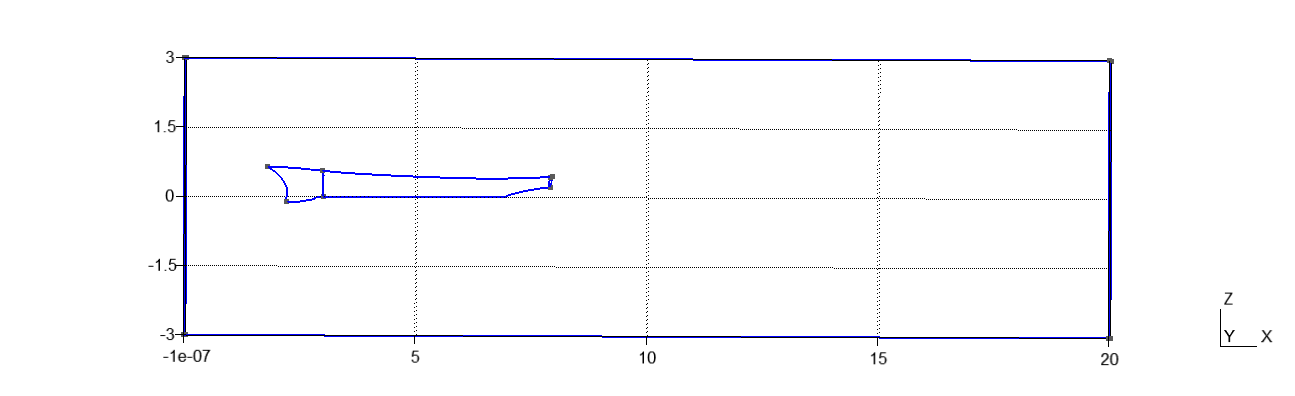
\includegraphics[width=1\textwidth]{domain_1.png}
    \caption{Side View of the Computational Domain}
\end{figure}
\begin{figure}[ht]
    \centering
    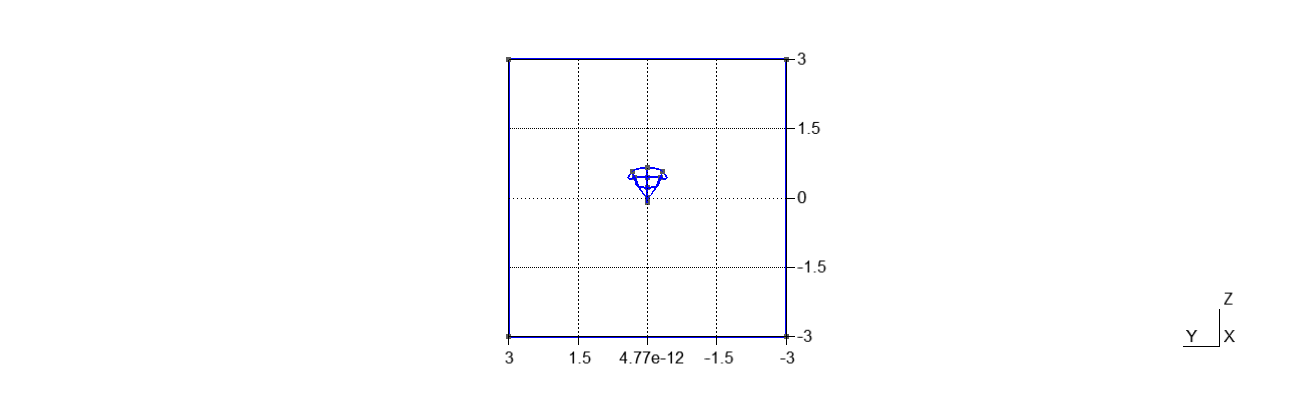
\includegraphics[width=1\textwidth]{domain_2.png}
    \caption{Front View of the Computational Domain}
\end{figure}
\begin{figure}[ht]
    \centering
    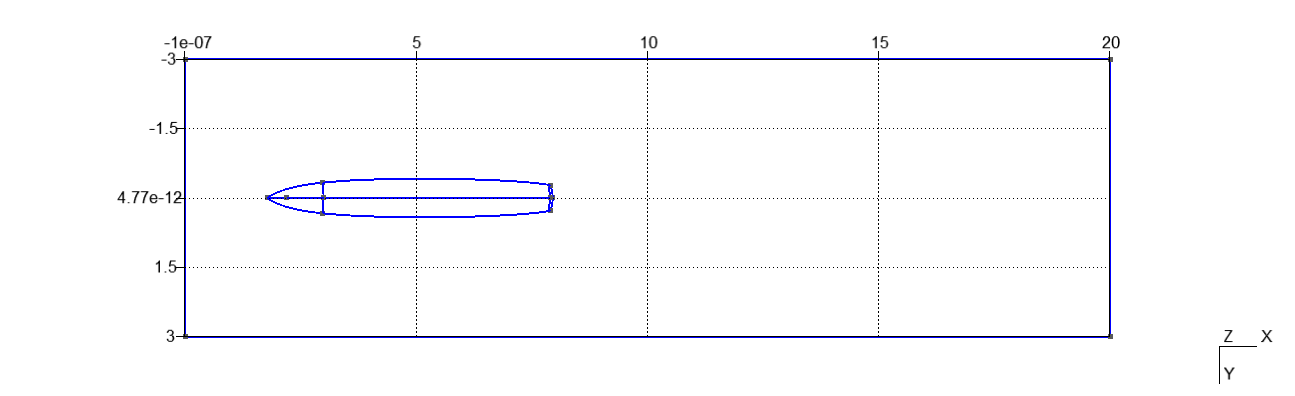
\includegraphics[width=1\textwidth]{domain_3.png}
    \caption{Top View of the Computational Domain}
\end{figure}

\clearpage
\section*{Appendix C}
\begin{lstlisting}[language=C, caption={Hard code for inlet wave run-up}, label={lst:wave_runup}, basicstyle=\ttfamily\footnotesize, keywordstyle=\color{blue}, commentstyle=\color{green}, numbers=left, numberstyle=\tiny\color{gray}, breaklines=true]
    H_wave = 0.1144;          /* Wave height */
    D_water = 3.248;        /* Water depth */
    T_wave = 1.343;       /* Wave period */
    L_wave = 6.175;          /* Wave length */
    PI = 3.14159265 ;
    G = 9.81 ;
    
    // For Nonlinear second-order Stokes waves //
    
    if (solNbcHd->var == PRM_NBC_ORDER_PAR && solNbcHd->type == PRM_NBC_USR_DEF) {
        for (i=0; i<nNodes; i++) {
            time = rootHd->time + rootHd->timeInc;
            K_wave = 2*PI/L_wave;
            AA = cosh(K_wave * (crd[3*(nodes[i])+1] + D_water));
            BB = cosh(K_wave * D_water);
            CC = sinh(K_wave * D_water);
            FF = cosh(2.0*K_wave*D_water);
    
            A = H_wave/2.0;
            B = (PI*H_wave*H_wave/(8.0*L_wave))*(BB/pow(CC,3.0))*(2.0+FF);
            ss = (-A + sqrt(A*A+8*B*B))/(4*B);
            phase = 0.0 * acos(ss);
    
            DD = cos(-2.0 * PI * (time/T_wave));
            EE = cos(2.0*(-2.0*PI*(time/T_wave)));
            GG = cosh(2.0*(K_wave* (crd[3*(nodes[i])+1] + D_water)));
    
            LL = (H_wave/2.0)*DD + ((PI*H_wave*H_wave/(8.0*L_wave))*(BB/pow(CC,3.0))*(2.0+FF)*EE);
            values[i] = -tanh((crd[3*nodes[i]+2]-LL-0.248)/(sqrt(2) * rootHd->epsilon));
        }
    }
    \end{lstlisting}

\section*{Appendix D}
\begin{verbatim}
clc
clear all

F1 = fopen('domain.oisd','r');
N = 1100;
dt = 0.05 ;
time = [dt:dt:N*dt];
L_OA = 6.175;
B_OA = 0.83;
rho_w = 1002;
a = L_OA/100;

NO1 = 700;
NO2 = N;

Force = zeros(N, 3); 
Disp = zeros(N, 3); 
fgets(F1);

for i=1:N
    for j=1:8
        fgets(F1);
    end
    fgets(F1); 
    Force(i,:) = fscanf(F1, '%e %e %e', [1 3]);
    
    for j=1:8
        fgets(F1);
    end
    
end

fclose(F1);

%mean = sum(Force(NO1:NO2,3))/(NO2-NO1);

[pks, locs] = findpeaks(Force(NO1:NO2,3),time(NO1:NO2));

avg = sum(pks)/length(pks);

VSF = avg/(rho_w*9.81*L_OA*B_OA*a);
VSF_ref = 10/(1000*9.81*3*0.403*0.03);

err = abs(VSF-VSF_ref)/VSF_ref;


A = L_OA*10;
T = 1.34375;
w = 2*pi/T;
W = A*sin(w*time(NO1:NO2));

figure(1)
plot(time(NO1:NO2),Force(NO1:NO2,3),'-k');
hold on;
plot(time(NO1:NO2),W,'-r');
legend('Vertical Force(N)','Wave(mm)');
xlabel('Time(s)');
ylabel('Vertical Shear Force(N)');

disp(avg)
disp(VSF)
disp(err)

\end{verbatim}

\section*{Appendix E}
\begin{figure}[ht]
    \centering
    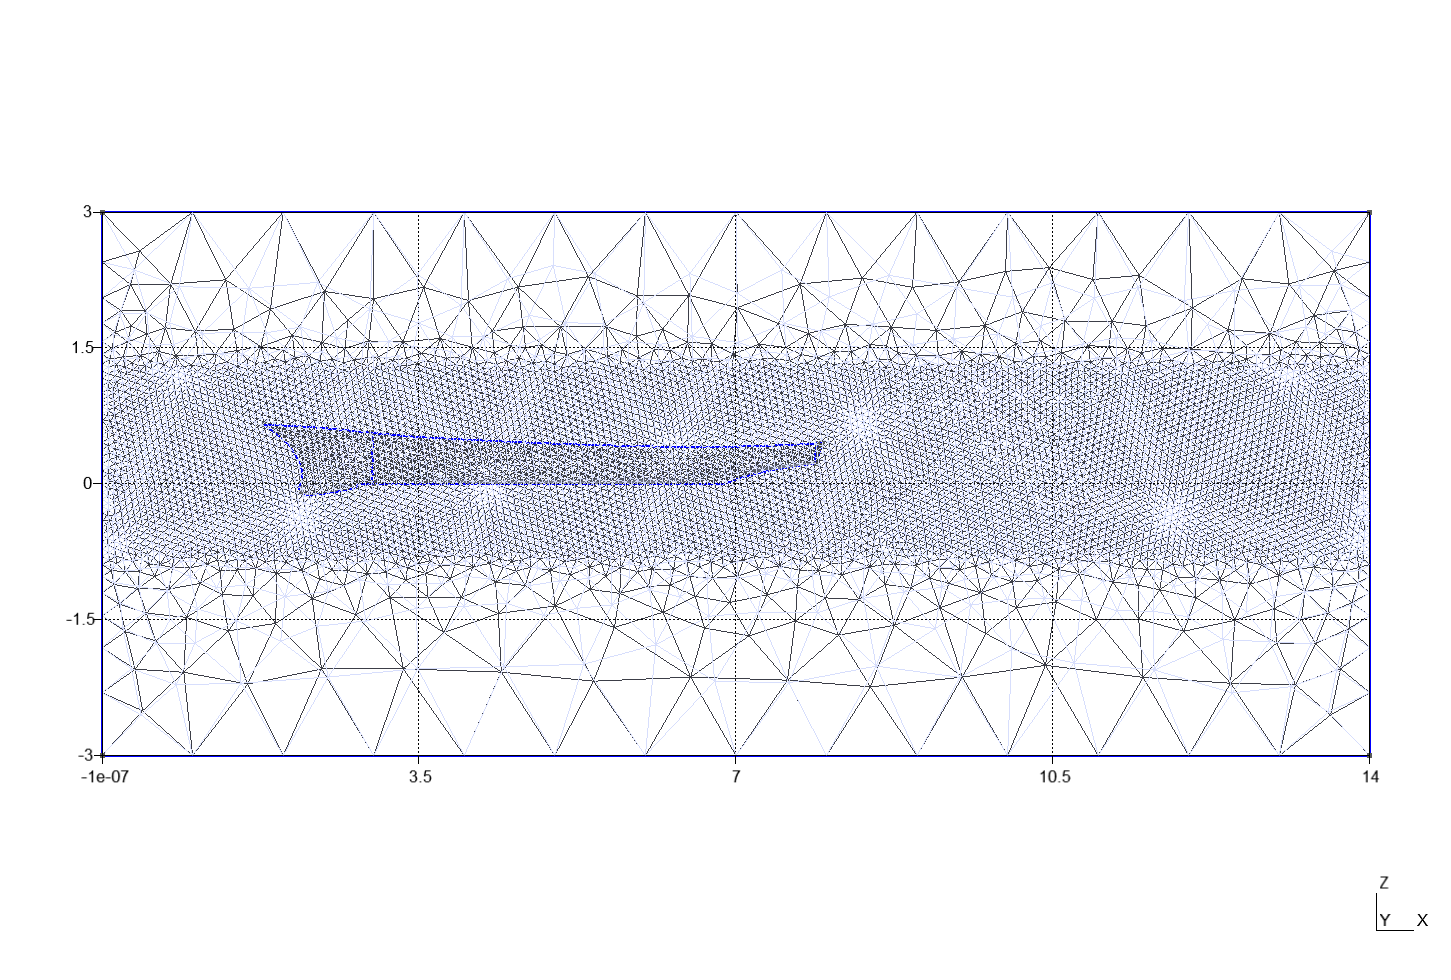
\includegraphics[width=1\textwidth]{Mesh_3.png}
    \caption{Side View of the Mesh}
\end{figure}
\begin{figure}[ht]
    \centering
    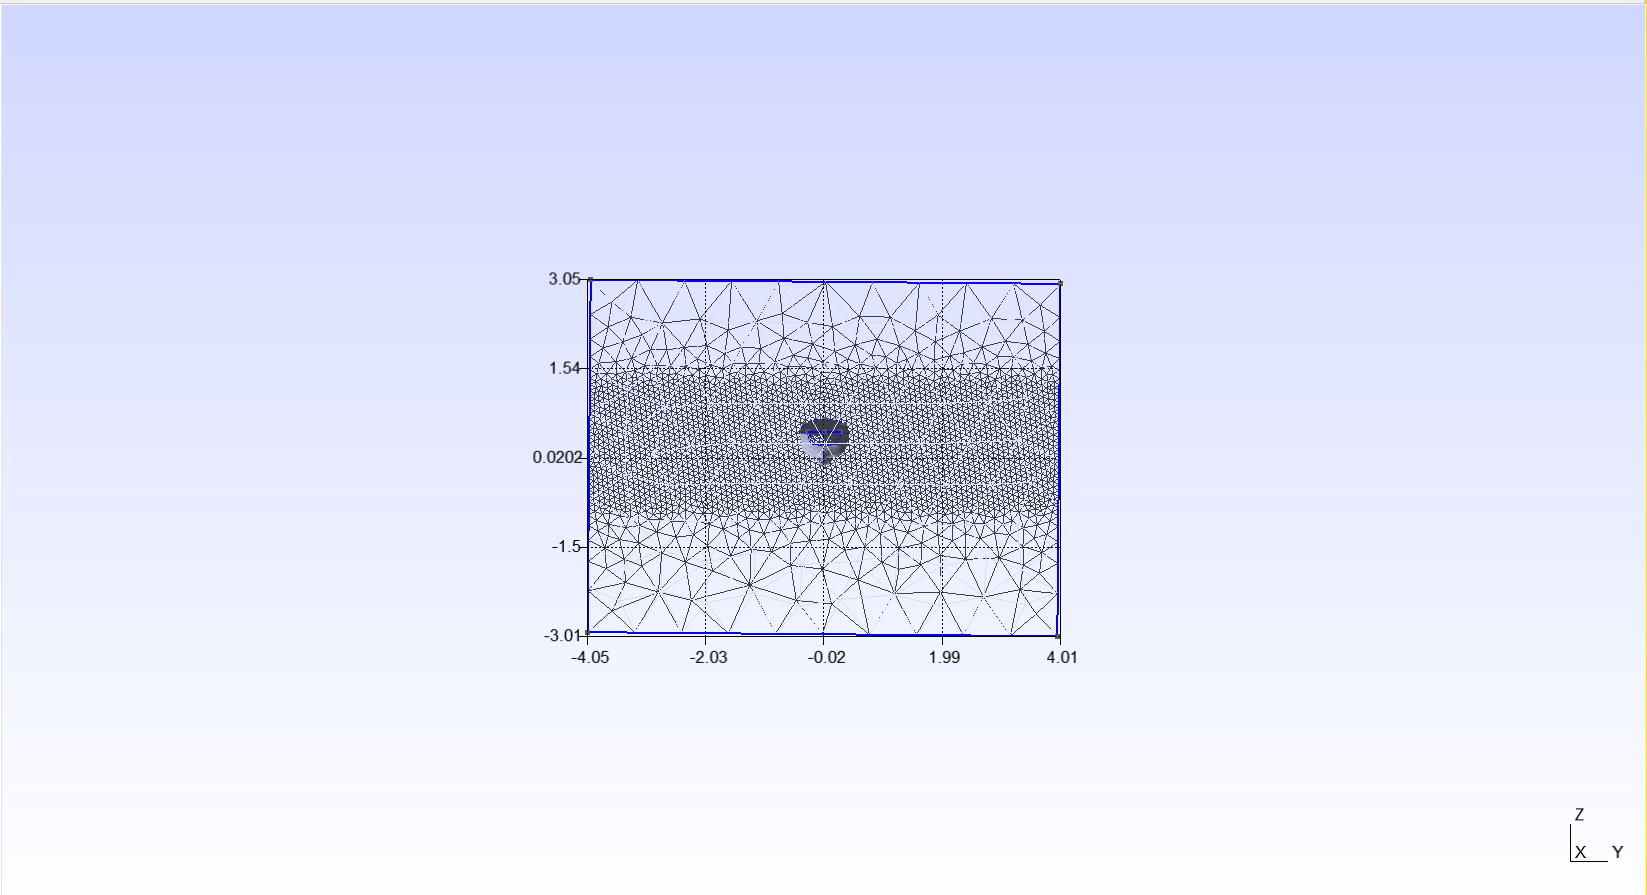
\includegraphics[width=1\textwidth]{Mesh_2.png}
    \caption{Front View of the Mesh}
\end{figure}
\begin{figure}[ht]
    \centering
    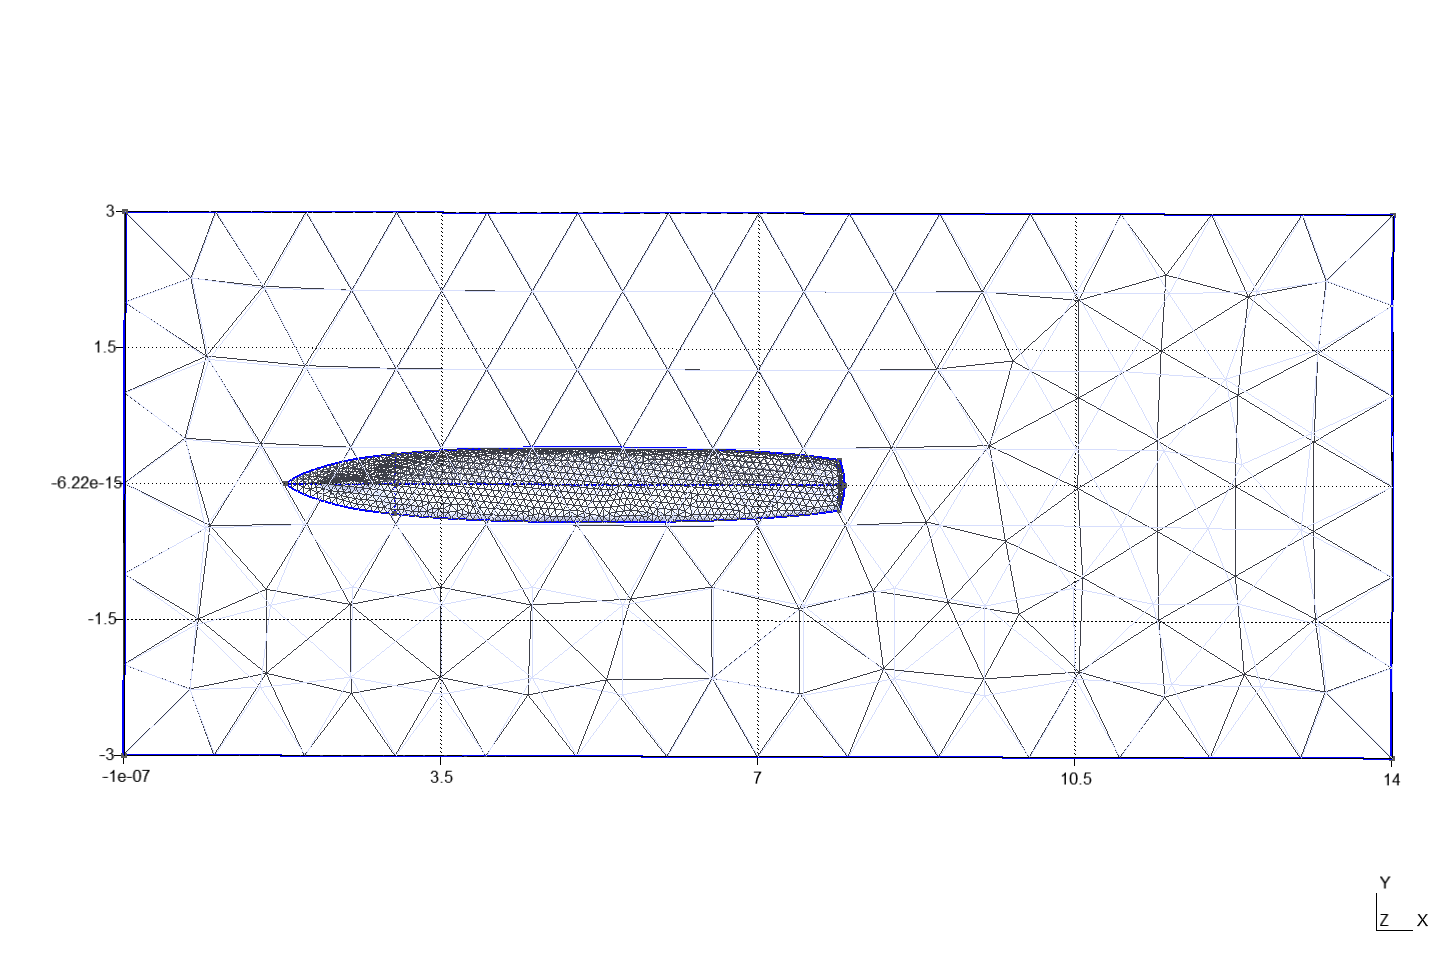
\includegraphics[width=1\textwidth]{Mesh_4.png}
    \caption{Top View of the Mesh}
\end{figure}
\begin{figure}[ht]
    \centering
    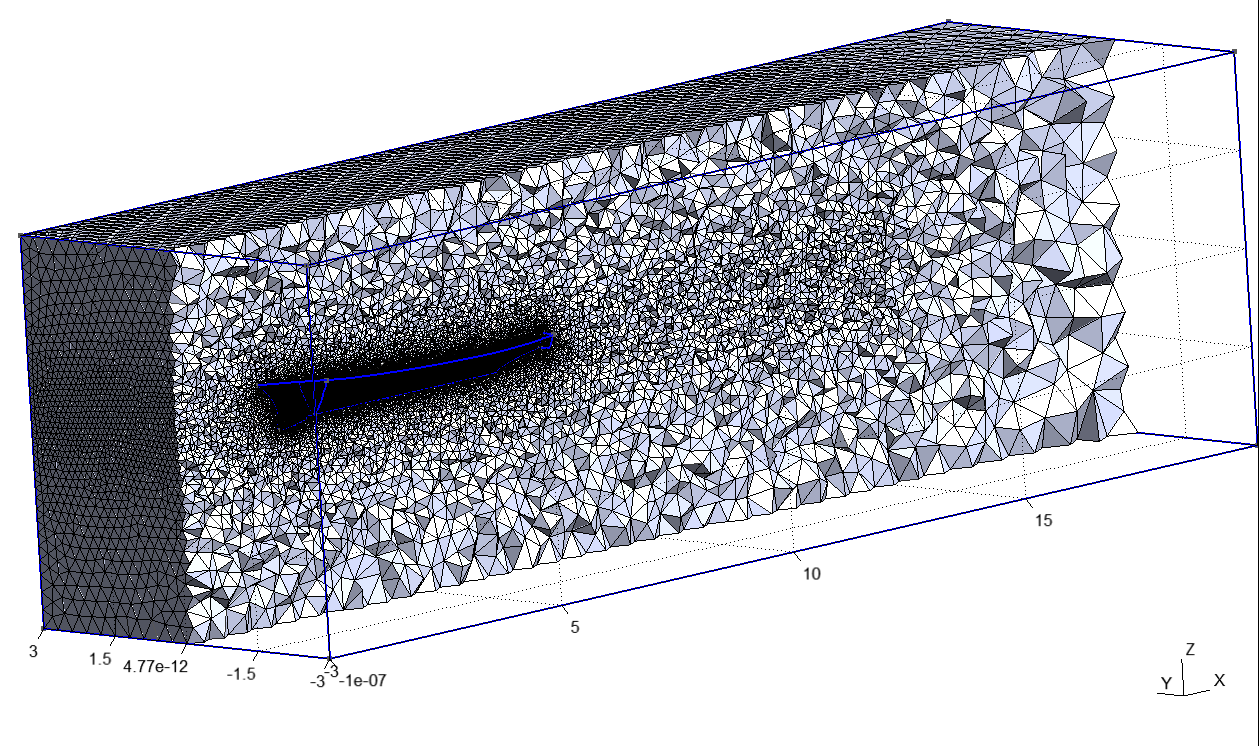
\includegraphics[width=1\textwidth]{Mesh_3D.png}
    \caption{3D View of the Mesh}
\end{figure}

\end{document}